\documentclass{article}
\usepackage[utf8]{inputenc}
\usepackage{authblk}
\usepackage{graphicx}
\usepackage{blindtext}
\usepackage{amsmath}
\usepackage{mathtools}
\usepackage{algorithm}
\usepackage{algpseudocode}
\usepackage{multirow}

\usepackage[dvipsnames]{xcolor}
\definecolor{faintBlue}{RGB}{233, 248, 255}
\definecolor{darkBlue}{RGB}{0, 65, 96}
	

\begin{document} 
\pagecolor{faintBlue}                                                   %PageColor is applied
                                                                        
                                                                        
                                                                        %Title, Author, Affiliation, Email, Date are mentioned
\title{CS213 Assignment on latex} 
\author{T Satwik \\ \texttt{190030043@iitdh.ac.in}}                     %Email is formatted using teletype font
\affil{Computer Science \& Engineering, IIT Dharwad}                       
\date{September 2, 2020}

\tableofcontents                                                        %Table of contents, List of figures, List of tables is specified
\listoffigures
\listoftables
                                                                        %references/bibliography is mentioned at the end
\begin{figure}                                                          %iit-logo(figure1) is referenced in the note mentioned below(cross Referencing)
    \centering
    
\includegraphics{college-logo.jpg}
    \caption{IIT Dharwad Logo}
    \label{fig:college-logo}
\end{figure}
\maketitle
                                                                    %in the below note text formatting is done, and text background and text colors are also changed.
\begin{center}
\textbf{\colorbox{darkBlue}{\textcolor{faintBlue}{Note: }}} \textit{Figure~\ref{fig:college-logo}, shows the logo of IIT Dharwad}    
\end{center}



\begin{table}                                                       %table 1 is specified
    \centering
    \begin{tabular}{| l| c |p{8cm} |}
        \hline
         sl. no & Section Name & Section Description \\
         \hline
         1 & Mathematical Expressions & Section~\ref{Mathematical} has examples of mathematical expressions  \\
         2 & Pseudo Code for Quick Sort & Section~\ref{Pseudo Code} has pseudo code for quick sort \\
         3 & Making Lists &  Section~\ref{Lists} has examples of lists\\
         \hline
         
    \end{tabular}
    \caption{Sections Table}
    \label{tab:Section table}
\end{table}

\clearpage
\section{Mathematical Expressions} \label{Mathematical}         %all sections are specified, labelled and also referenced in the above table
\subsection{Inline Mathematical Expression}                     %text color is changed and is formatted to bold face in the below line
This is the example for an \textbf{\textcolor{RoyalPurple}{inline mathematical expression}} $E=MC^2$ \cite{einstein1979general} 
                                                                %citation 1 is marked in the above code
                                                                
\subsection{Non numbered equation in a dedicated line}
This is the example for a \textbf{\textcolor{RoyalPurple}{non numbered equation in a dedicated line}} 
\begin{equation}
    Kinetic \ Energy = \frac{1}{2}mv^2 \nonumber
    \label{eq:KE}
\end{equation}

\subsection{Numbered equation in a dedicated line}
This is the example for a \textbf{\textcolor{RoyalPurple}{Numbered equation in a dedicated line}} 
\begin{equation}
    Gravitational \ Potential \ Energy = mgh
    \label{eq:GPU}                                              %Above Equation is labelled and referenced in a note later 
\end{equation}

\subsection{Multi-line Equation}
This is the example for a \textbf{\textcolor{RoyalPurple}{Multi-line Equation}}  
\begin{eqnarray}
    W &=& \Vec{F}.\Vec{S} \nonumber\\
      &=& FS\cos\theta \nonumber
\end{eqnarray}

\subsection{Matrices}
This is the example for \textbf{\textcolor{RoyalPurple}{Matrices}}
\begin{eqnarray}
Identity \ Matrix = 
   \begin{bmatrix}
    1 & 0 \\
    0 & 1 
    \end{bmatrix} \nonumber\\
Null \ Matrix = 
    \begin{bmatrix}
    0 & 0 \\
    0 & 0 
    \end{bmatrix} \nonumber
\end{eqnarray}

\subsection{Square root, Summation, Integration, Nested Brackets, Fractions}

This is an example for a equation with \textbf{\textcolor{RoyalPurple}{Square root}}
\begin{equation}
 Magnitude \ of \  a \ vector \ \Vec{a} = \sqrt{a_x^2 + a_y^2 + a_z^2 }  \nonumber 
\end{equation}

This is an example for a equation with \textbf{\textcolor{RoyalPurple}{Summation and fractions}}
\begin{equation}
 Sum \ of \  first \ n \ natural \ numbers = \sum_{i=1}^n i = \frac{n(n+1)}{2} \nonumber 
\end{equation}

This is an example for a equation with \textbf{\textcolor{RoyalPurple}{Integration}}.
\begin{equation}
 Integral \ of \  f(x) \ over \ a \ to\ b = \int_{a}^b f(x)dx \nonumber  \nonumber 
\end{equation}

This is an example for a equation with \textbf{\textcolor{RoyalPurple}{Nested Brackets}}
\begin{equation}
 Distributive \ law : \bigg(  a (b+c) \bigg) = \bigg( (ab) + (ac) \bigg) \nonumber
\end{equation} 

\textbf{\colorbox{darkBlue}{\textcolor{faintBlue}{Note: }}} \textit{Equation~\ref{eq:GPU}, describes the Gravitational Potential Energy}  

\begin{figure}[h]                                               %figure 2 and 3 are specified and labelled
    \centering
    
\includegraphics[width=9cm]{Math-1.jpg}
    \caption{Mathematics Image 1}
    \label{fig:math-1}
\end{figure}
\begin{figure}[h]
    \centering
    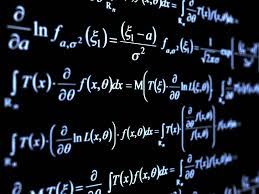
\includegraphics[width=9cm]{Math-2.jpg}
    \caption{Mathematics Image 2}
    \label{fig:math-2}
\end{figure}






\clearpage
\section {Pseudo Code for Quick Sort} \label{Pseudo Code}   %Quick Sort pseudo code section
\begin{algorithm}
\caption{Quick Sort Algorithm}
\begin{algorithmic}[1]

\Function{QuickSort}{$Arr, StartIndex, EndIndex$}{
    \If{$StartIndex < EndIndex$}
        \State $PivotIndex \gets \Call{Partition}{Arr, StartIndex, EndIndex}$
        \State $\Call{Quicksort}{Arr, StartIndex, PivotIndex-1}$
        \State $\Call{Quicksort}{Arr, PivotIndex+1, EndIndex}$
    \Else
        \State $ \Return $
    \EndIf
\EndFunction
} \\

\Function{Partition}{$Arr, StartIndex, EndIndex$}{
    \State $Pivot \gets Arr[EndIndex] $ 
    \State $PivotIndex  \gets StartIndex $ 
    \For{$i \gets StartIndex$ to $EndIndex-1$}
        \If{$Arr[i] <= Pivot$}
            \State $\Call{Swap}{Arr[i], Arr[PivotIndex]}$
            \State $PivotIndex \gets PivotIndex + 1$
        \EndIf
    \EndFor
    \State $\Call{Swap}{Arr[PivotIndex], Arr[EndIndex]}$ 
    \State $\Return \ PivotIndex $
\EndFunction     
} \\

\Function{Swap}{Arr[i], Arr[j]}{
    \State $temp \gets Arr[i]$
    \State $Arr[i] \gets Arr[j]$
    \State $Arr[j] \gets temp$
    \State $\Return$
\EndFunction
}\\
\end{algorithmic}
\end{algorithm}


\begin{figure}[h]                               %figure 4 is labelled and referenced in the note below
    \centering
    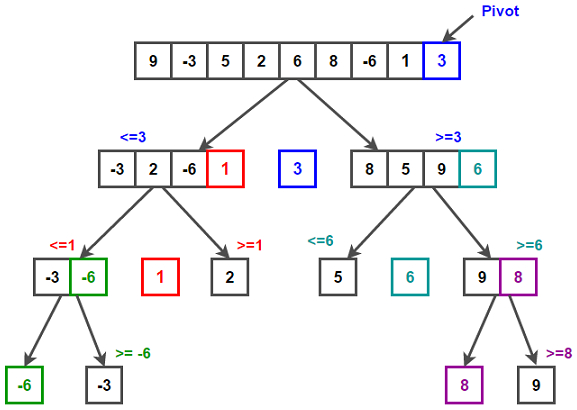
\includegraphics[width=10cm]{Quicksort.png}
    \caption{Quick Sort Image}
    \label{fig:Quicksort}
\end{figure}

\textbf{\colorbox{darkBlue}{\textcolor{faintBlue}{Note: }}}\textit{Refer to Figure~\ref{fig:Quicksort}, to see a detailed example of how Quick Sort works}
\textbf{\colorbox{darkBlue}{\textcolor{faintBlue}{Note: }}}\textit{Refer to \cite{10.1093/comjnl/5.1.10} and \cite{10.1145/359619.359631}, to learn more about Quick Sort}\\
\textbf{\colorbox{darkBlue}{\textcolor{faintBlue}{Note: }}}\textit{Refer to \cite{10.1145/146370.146381} and \cite{satish2009designing}, to know more about the other sorting algorithms}\\
    
                                            % in the notes above the image is referenced and 4 citations are linked to various papers on quick sort and other sorting methods        
    
    
\clearpage

\section{Making Lists}  \label{Lists}       %in this section various types of lists are illustrated 
The following are the different types of list items:
\subsection{Itemize}
\begin{itemize}
    \item The first point with Itemize style of formatting.
    \item The second point with Itemize style of formatting.
\end{itemize}

\subsection{Enumerate}
\begin{enumerate}
    \item The first point with Enumerate style of formatting.
    \item The second point with Enumerate style of formatting.
\end{enumerate}

\subsection{Description}
\begin{description}
    \item [\tab The First Point] The first point with Description style of formatting.
    \item [\tab The Second Point] The second point with Description style of formatting.
\end{description}


\begin{table}                   %In this table the various types of lists are described
    \centering
    \begin{tabular}{| l| c |p{5cm} |}
        \hline
         sl. no & List Type & Description \\
         \hline
         1 & itemize & The lists are not ordered and each point is marked by a dot. \\
         1 & enumerate & The lists are ordered and each point is marked by a number automatically. \\
         1 & description & The lists are not ordered and each point is marked by a word you specify in "[ ]". \\
         \hline
         
    \end{tabular}
    \caption{Types of list}
    \label{tab:Types of lists}
\end{table}

\textbf{\colorbox{darkBlue}{\textcolor{faintBlue}{Note: }}}\textit{In Table~\ref{tab:Types of lists}, we have described the types of list in tabular form.}


\bibliographystyle{plain}           %bibliography/references is specified
\bibliography{References}

\end{document}
